\documentclass{article}
\usepackage{graphicx}
\usepackage[dvipsnames,table]{xcolor}
\usepackage[utf8]{inputenc}
\usepackage{siunitx}
\usepackage[american,siunitx]{circuitikz}
\usepackage{amsmath}
\usepackage{svg}
\usepackage{booktabs}
\usepackage{float}
\usepackage{xparse, xfp}
\usepackage{multirow}
\usepackage{tikz}
\usepackage{karnaugh-map}
\usepackage{pdfpages}
\usepackage{hyperref}
\hypersetup{
    colorlinks=true,
    linkcolor=blue,
    filecolor=magenta,      
    urlcolor=cyan,
}
\usetikzlibrary{calc}
%\usepackage[landscape]{geometry}
\renewcommand{\thesubsection}{\thesection.\alph{subsection}}
\newcommand{\equal}{=}
\newcommand{\greyrule}{\arrayrulecolor{black!30}\midrule\arrayrulecolor{black}}
\makeatletter
\newcommand\currcoor{\the\tikz@lastxsaved,\the\tikz@lastysaved}
\makeatother
\newcolumntype{:}{@{\hskip\tabcolsep\color{black!30}\vrule\hskip\tabcolsep}}

\ExplSyntaxOn
\NewExpandableDocumentCommand \groupify { O{\,\allowbreak} m m }
  { \jakob_groupify:nnn {#1} {#2} {#3} }
\cs_new:Npn \jakob_groupify:nnn #1 #2 #3
  { \__jakob_groupify_loop:nnw { 1 } {#2} #3 \q_recursion_tail {#1} \q_recursion_stop }
\cs_new:Npn \__jakob_groupify_loop:nnw #1 #2 #3
  {
    \quark_if_recursion_tail_stop:n {#3}
    \exp_not:n {#3}
    \int_compare:nNnTF {#1} = {#2}
      { \__jakob_groupify_sep:n }
      { \exp_args:Nf \__jakob_groupify_loop:nnw { \int_eval:n { #1+1 } } }
          {#2}
  }
\cs_new:Npn \__jakob_groupify_sep:n #1 #2 \q_recursion_tail #3
  {
    \tl_if_empty:nF {#2} { \exp_not:n {#3} }
    \__jakob_groupify_loop:nnw { 1 } {#1}
    #2 \q_recursion_tail {#3}
  }
\ExplSyntaxOff

\title{ECE 2300L\\Digital Logic Design Laboratory\\\,\\Experiment 12\\\,\\Report}
\author{Choi Tim Antony Yung}
\begin{document}
\maketitle

\thispagestyle{empty}
\setcounter{page}{0}

\newpage

\section*{Pulse Generator Using 555 Timer}
\begin{center}
  \begin{circuitikz}
    \draw
    (0,0) node[dipchip,num pins=8,hide numbers,external pins width=0.0](timer){}
    (timer.bpin 1) node[right]{1}
    (timer.bpin 2) node[right]{2}
    (timer.bpin 3) node[right]{3}
    (timer.bpin 4) node[right]{4}
    (timer.bpin 5) node[left]{5}
    (timer.bpin 6) node[left]{6}
    (timer.bpin 7) node[left]{7}
    (timer.bpin 8) node[left]{8}

    (timer.bpin 1) -- ++(-0.5,0) -- ++(0,-0.1) node[tlground]{}
    (timer.bpin 2) -- ++(-1,0) -- ++(0,-4) node[circ](cgnd){} -- (\currcoor -| timer.bpin 6) -- ++(2.5,0) -- ++(0,6) -- (\currcoor -| timer.bpin 8) to[R=\SI{1}{\mega\ohm}] (\currcoor -| timer.bpin 1) -- ++(-2,0) -- (\currcoor |- timer.bpin 3) node[circ]{} -- ++(-1,0) node[left]{CLK}
    (timer.bpin 3) ++(-2,0) to[crossing] ++(2,0)
    (timer.bpin 4) -- ++(-0.5,0) node[vcc]{} node[below]{5V}
    (timer.bpin 5) -- ++(0.5,0) -- ++(0,-0.5) to[C=\SI{100}{\nano\farad}] ++(0,-1) node[ground]{}
    (timer.bpin 6) -- ++(2.5,0) node[circ]{}
    (timer.bpin 8) -- ++(0.5,0) node[vcc]{5V}
    (cgnd) -- ++(0,-0.5) to[C=\SI{10}{\nano\farad}] ++(0,-1) node[ground]{}
    ;
  \end{circuitikz}
\end{center}

\section*{Pulse Generator Using Inverter}
\begin{center}
  \begin{circuitikz}
    \draw
    (0,0) -- ++(0.5,0) node[not port, anchor=in](not1){}
    (not1.out) -- ++(0.5,0) node[not port, anchor=in](not2){}
    (not2.out) -- ++(0.5,0) node[not port, anchor=in](not3){}
    (0,0) -- ++(0,1) node[circ]{} to[C=\SI{10}{\nano\farad}] (\currcoor -| not2.out) -- ++(0.25,0)  -- ++(0,-1) node[circ]{}
    (0,0) ++(0,1) -- ++(0,1) -- ++(1,0) to[R=\SI{6.6}{\kilo\ohm}] (\currcoor -| not3.out) -- ++(0.25,0) -- ++(0,-2) node[circ]{}
    (not3.out) -- ++(0.75,0) node[right]{CLK}
    ;
    \draw [color=red]
    (not1.in) node[below]{1}
    (not1.out) node[below left]{2}
    (not2.in) node[below]{3}
    (not2.out) node[below left]{4}
    (not3.in) node[below]{5}
    (not3.out) node[below left]{6}
    ;
  \end{circuitikz}
\end{center}
\newpage

\section*{State Diagram}
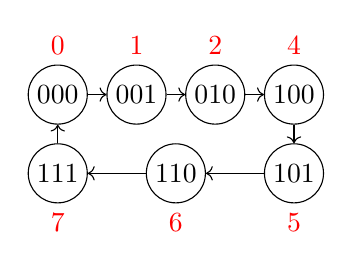
\begin{tikzpicture}
  \node(a)[draw,circle,minimum size=0.75cm,inner sep=0pt] at (0,0) {$000$};
  \node(b)[draw,circle,minimum size=0.75cm,inner sep=0pt] at (1,0) {$001$};
  \node(c)[draw,circle,minimum size=0.75cm,inner sep=0pt] at (2,0) {$010$};
  \node(d)[draw,circle,minimum size=0.75cm,inner sep=0pt] at (3,0) {$100$};
  \node(e)[draw,circle,minimum size=0.75cm,inner sep=0pt] at (3,-1) {$101$};
  \node(f)[draw,circle,minimum size=0.75cm,inner sep=0pt] at (1.5,-1) {$110$};
  \node(g)[draw,circle,minimum size=0.75cm,inner sep=0pt] at (0,-1) {$111$};

  \draw [->] (a.0) -- (b.180);
  \draw [->] (b.0) -- (c.180);
  \draw [->] (c.0) -- (d.180);
  \draw [->] (d.270) -- (e.90);
  \draw [->] (e.180) -- (f.0);
  \draw [->] (f.180) -- (g.0);
  \draw [->] (g.90) -- (a.270);

  \draw[color=red] (a.90) node[above]{0};
  \draw[color=red] (b.90) node[above]{1};
  \draw[color=red] (c.90) node[above]{2};
  \draw[color=red] (d.90) node[above]{4};
  \draw[color=red] (e.270) node[below]{5};
  \draw[color=red] (f.270) node[below]{6};
  \draw[color=red] (g.270) node[below]{7};


\end{tikzpicture}

\section*{State Table}
\begin{table}[H]
  \begin{tabular}{ccc|ccc|ccc}
      \toprule
      $A$&$B$&$C$&$A^+$&$B^+$&$C^+$&$T_A$&$T_B$&$T_C$\\
      \midrule
      0&0&0 & 0&0&1 & 0&0&1\\
      0&0&1 & 0&1&0 & 0&1&1\\
      0&1&0 & 1&0&0 & 1&1&0\\
      1&0&0 & 1&0&1 & 0&0&1\\
      1&0&1 & 1&1&0 & 0&1&1\\
      1&1&0 & 1&1&1 & 0&0&1\\
      1&1&1 & 0&0&0 & 1&1&1\\
      \bottomrule
  \end{tabular}
\end{table}

\section*{Truth Table}
\begin{table}[H]
  \begin{tabular}{ccc|c}
    \toprule
    $A$&$B$&$C$&$T_A$\\
    \midrule
    0&0&0 & 0\\
    0&0&1 & 0\\
    0&1&0 & 1\\
    1&0&0 & 0\\
    1&0&1 & 0\\
    1&1&0 & 0\\
    1&1&1 & 1\\
    \bottomrule
  \end{tabular}
  \quad
  \begin{tabular}{ccc|c}
    \toprule
    $A$&$B$&$C$&$T_B$\\
    \midrule
    0&0&0 & 0\\
    0&0&1 & 1\\
    0&1&0 & 1\\
    1&0&0 & 0\\
    1&0&1 & 1\\
    1&1&0 & 0\\
    1&1&1 & 1\\
    \bottomrule
  \end{tabular}
  \quad
  \begin{tabular}{ccc|c}
    \toprule
    $A$&$B$&$C$&$T_C$\\
    \midrule
    0&0&0 & 1\\
    0&0&1 & 1\\
    0&1&0 & 0\\
    1&0&0 & 1\\
    1&0&1 & 1\\
    1&1&0 & 1\\
    1&1&1 & 1\\
    \bottomrule
  \end{tabular}
\end{table}
\newpage

\section*{Karnaugh Maps}
\begin{table}[H]
  \begin{tabular}{cc}
    \begin{karnaugh-map}[4][2][1][$BC$][$A$]
      \minterms{2,7}
      \terms{3}{X}
      \implicant{3}{7}
      \implicant{3}{2}
    \end{karnaugh-map}
    &
    \begin{karnaugh-map}[4][2][1][$BC$][$A$]
      \minterms{1,2,5,7}
      \terms{3}{X}
      \implicant{1}{7}
      \implicant{3}{2}
    \end{karnaugh-map}
    \\
    $T_A=\textcolor{red}{BC}+\textcolor{Green}{\overline{A}B}$&$T_B=\textcolor{red}{C}+\textcolor{Green}{\overline{A}B}$\\
  \end{tabular}
\end{table}
\begin{center}
\begin{karnaugh-map}[4][2][1][$BC$][$A$]
  \minterms{0,1,4,5,6,7}
  \terms{3}{X}
  \implicant{4}{6}
  \implicant{0}{5}
\end{karnaugh-map}
\end{center}
$$T_C=\textcolor{red}{A}+\textcolor{Green}{\overline{B}}$$
\newpage

\section*{Schematic}
\begin{center}
    \begin{circuitikz}
      \draw (0,0) node[dipchip,num pins=8,hide numbers,external pins width=0.0](decoder){};
      \draw (decoder.east) -- ++(0.5,0) node[above]{$a-g$} -- ++(0.5,0) node[seven segment val=8 dot none box on, anchor=west]{};
      \draw (decoder.bpin 1) node[right]{6} -- ++(-0.5,0) coordinate(d3) node[above]{$d_3$};
      \draw (decoder.bpin 2) node[right]{2} -- ++(-0.5,0) coordinate(d2) node[above]{$d_2$};
      \draw (decoder.bpin 3) node[right]{1} -- ++(-0.5,0) coordinate(d1) node[above]{$d_1$};
      \draw (decoder.bpin 4) node[right]{7} -- ++(-0.5,0) coordinate(d0) node[above]{$d_0$};
      \draw (decoder.bpin 1) ++(-0.5,0) -- ++(-0.5,0) -- ++(0,-0.2) node[tlground]{};
      \draw (decoder.bpin 2) ++(-0.5,0) ++(-2.5,-5) node[flipflop JK, anchor=pin 6](JKA){};
      \draw (decoder.bpin 3) ++(-0.5,0) ++(0,-2.5) ++(-2.5,-5) node[flipflop JK, anchor=pin 6](JKB){};
      \draw (decoder.bpin 3) ++(-0.5,0) ++(0,-5.5) ++(-2.5,-5) node[flipflop JK, anchor=pin 6](JKC){};
      \draw (JKA.pin 1) -- ++(-0.5,0) coordinate(TA) node[above]{$T_A$} -- (\currcoor|-JKA.pin 3) -- ++(0.3,0) to[crossing]++(0.2,0);
      \draw (JKB.pin 1) ++(-0.5,0) -- ++(0.3,0) to[crossing]++(0.2,0) ++(-0.5,0) coordinate(TB) node[above]{$T_B$} -- (\currcoor|-JKB.pin 3) -- ++(0.3,0) to[crossing]++(0.2,0);
      \draw (JKC.pin 1) ++(-0.5,0) -- ++(0.3,0) to[crossing]++(0.2,0) ++(-0.5,0) coordinate(TC) node[above]{$T_C$} -- (\currcoor|-JKC.pin 3) -- ++(0.3,0) to[crossing]++(0.2,0);
      \draw (JKA.pin 2) -- ++(-0.1,0) -- (\currcoor|-JKC.pin 3) -- ++(0,-1) node[below]{CLK};
      \draw (JKB.pin 2) -- ++(-0.1,0);
      \draw (JKC.pin 2) -- ++(-0.1,0);

      \draw [color=red] (JKA.pin 6) coordinate(A) node[below]{$A$};
      \draw [color=cyan] (JKA.pin 4) coordinate(notA) node[below]{$\overline{A}$};
      \draw [color=green] (JKB.pin 6) coordinate(B) node[below]{$B$};
      \draw [color=magenta] (JKB.pin 4) coordinate(notB) node[below]{$\overline{B}$};
      \draw [color=blue] (JKC.pin 6) coordinate(C) node[below]{$C$};
      \draw (JKC.pin 4) coordinate(notC) node[below]{$\overline{C}$};

      \draw 
      (TA) -- ++(-0.5,0) node[or port, anchor=out,rotate=270](aor){}
      (aor.in 1) -- ++(0.5,0) node[and port, anchor=out,rotate=270](and1){}
      (TB) -- ++(-1.75,0) node[or port, anchor=out,rotate=270](bor){}
      (aor.in 2) -- ++(-0.5,0) node[and port, anchor=out,rotate=270](and2){} -- (\currcoor-|bor.in 1) -- (bor.in 1)
      (TC) -- ++(-3,0) node[or port, anchor=out,rotate=270](cor){}
      (aor.in 2) node[above]{$\textcolor{cyan}{\overline{A}}\textcolor{green}{B}$}
      (bor.in 1) node[right]{$\textcolor{cyan}{\overline{A}}\textcolor{green}{B}$}
      (cor.out) node[below]{$\textcolor{red}{A}+\textcolor{magenta}{\overline{B}}$}
      (and1.out) node[right]{$\textcolor{green}{B}\textcolor{blue}{C}$}
      (aor.out) node[below]{$\scriptstyle{\textcolor{cyan}{\overline{A}}\textcolor{green}{B}+\textcolor{green}{B}\textcolor{blue}{C}}$}
      (bor.out) node[below]{$\textcolor{blue}{C}+\textcolor{cyan}{\overline{A}}\textcolor{green}{B}$}


      ;

      \draw [color=red]
      (A) -- (A|-d2)
      (d2) -- (d2-|cor.in 2) -- (cor.in 2)
      ;

      \draw [color=cyan]
      (notA) -- ++(0.5,0) -- (\currcoor|-d1) -- ++(0,0.275) -- (\currcoor-|and2.in 2) -- (and2.in 2)
      ;

      \draw [color=green]
      (B) -- ++(1,0) -- (\currcoor|-d1)
      (d1) -- (d1-|and2.in 1) -- (and2.in 1)
      (and1.in 2) -- (and1.in 2 |- d1)
      ;

      \draw [color=magenta]
      (notB) -- ++(1.5,0) -- (\currcoor|-d0) -- ++(0,0.275) -- (\currcoor-|cor.in 1) -- (cor.in 1)
      ;

      \draw [color=blue]
      (C) -- ++(2,0) -- (\currcoor|-d0)
      (d0) -- (d0-|bor.in 2) -- (bor.in 2)
      (and1.in 1) -- (and1.in 1 |- d0)
      ;

      % pinout
      \draw [color=red]
      (JKA.bpin 1) ++(0.3,0) node[right]{7}
      (JKA.bpin 2) ++(0.3,0) node[right]{5}
      (JKA.bpin 3) ++(0.3,0) node[right]{10}
      (JKA.bpin 4) ++(-0.3,0) node[left]{8}
      (JKA.bpin 6) ++(-0.3,0) node[left]{9}
      (JKB.bpin 1) ++(0.3,0) node[right]{14}
      (JKB.bpin 2) ++(0.3,0) node[right]{1}
      (JKB.bpin 3) ++(0.3,0) node[right]{3}
      (JKB.bpin 4) ++(-0.3,0) node[left]{13}
      (JKB.bpin 6) ++(-0.3,0) node[left]{12}
      (JKC.bpin 1) ++(0.3,0) node[right]{7}
      (JKC.bpin 2) ++(0.3,0) node[right]{5}
      (JKC.bpin 3) ++(0.3,0) node[right]{10}
      (JKC.bpin 4) ++(-0.3,0) node[left]{8}
      (JKC.bpin 6) ++(-0.3,0) node[left]{9}
      ;
    \end{circuitikz}
\end{center}

\newpage

\section*{Demo}
Video demonstrations can be found \href{https://photos.app.goo.gl/eSdNj98HEJmizMVE7}{here} at \url{https://photos.app.goo.gl/eSdNj98HEJmizMVE7}
\subsubsection*{Pulse Generator}
\begin{figure}[ht!]
  \centering
  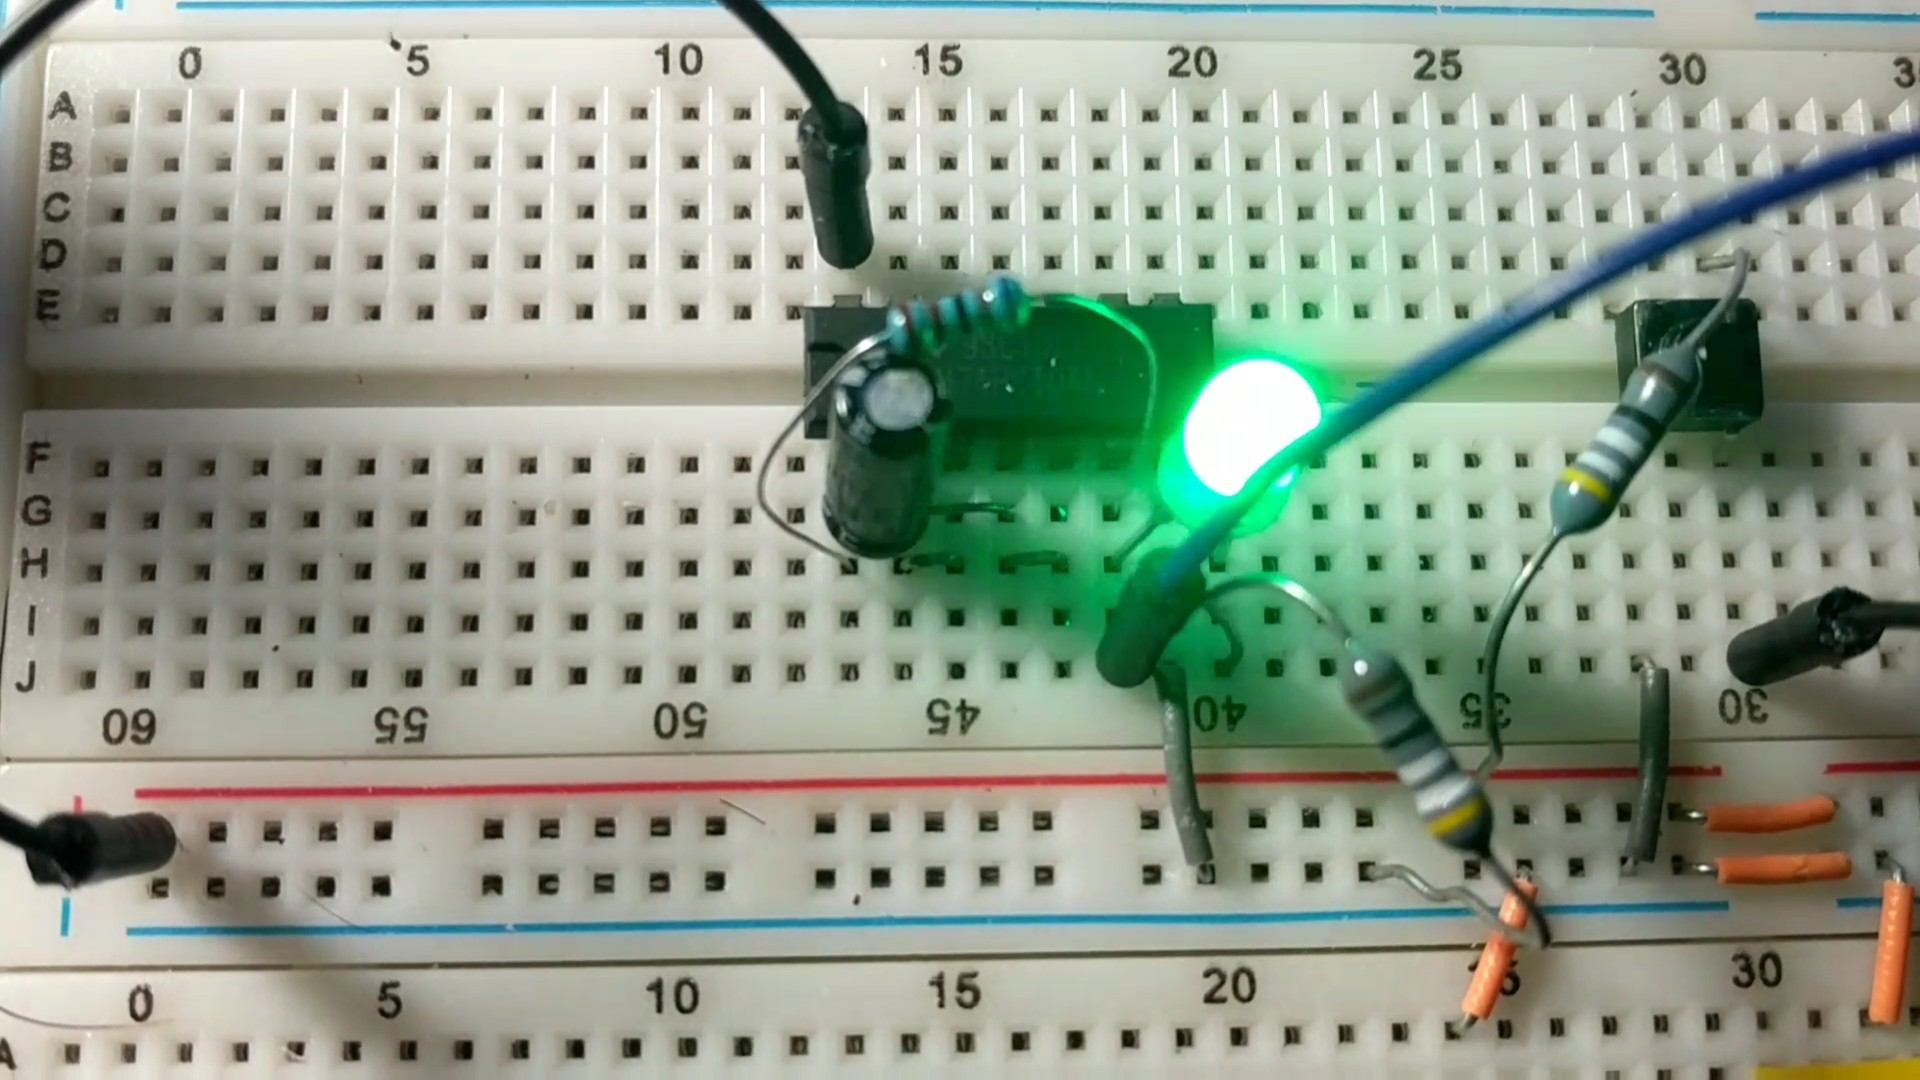
\includegraphics[width=\textwidth]{ECE2300L_Lab12_Pulse.jpg}
\end{figure}
\begin{figure}[ht!]
  \centering
  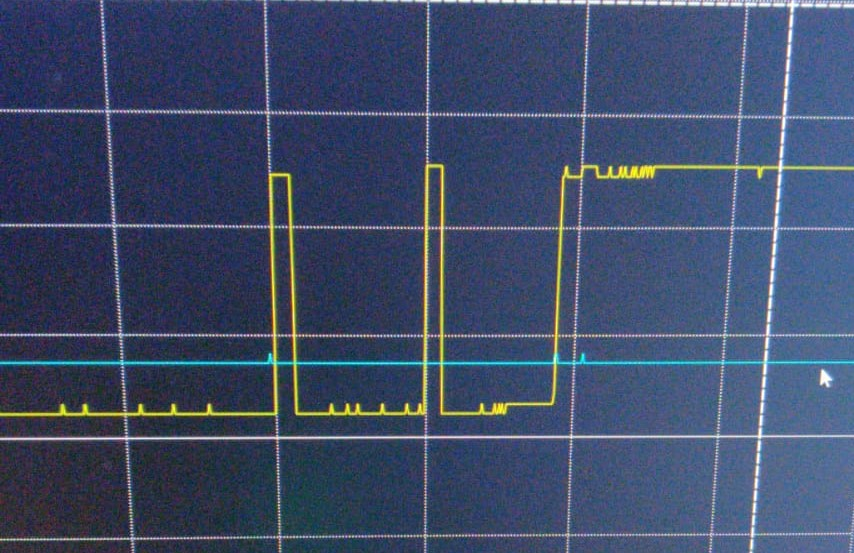
\includegraphics[width=0.95\textwidth]{ECE2300L_Lab12_PulseStart.jpeg}
\end{figure}
As seen from the oscilloscope capture above, the pulse generator have multiple rising edges at the start of the pulse, therefore it is not suitable to be used as clock. For the counter, a push button was used instead.

\newpage
\subsubsection*{Counter}
\begin{figure}[ht!]
  \centering
  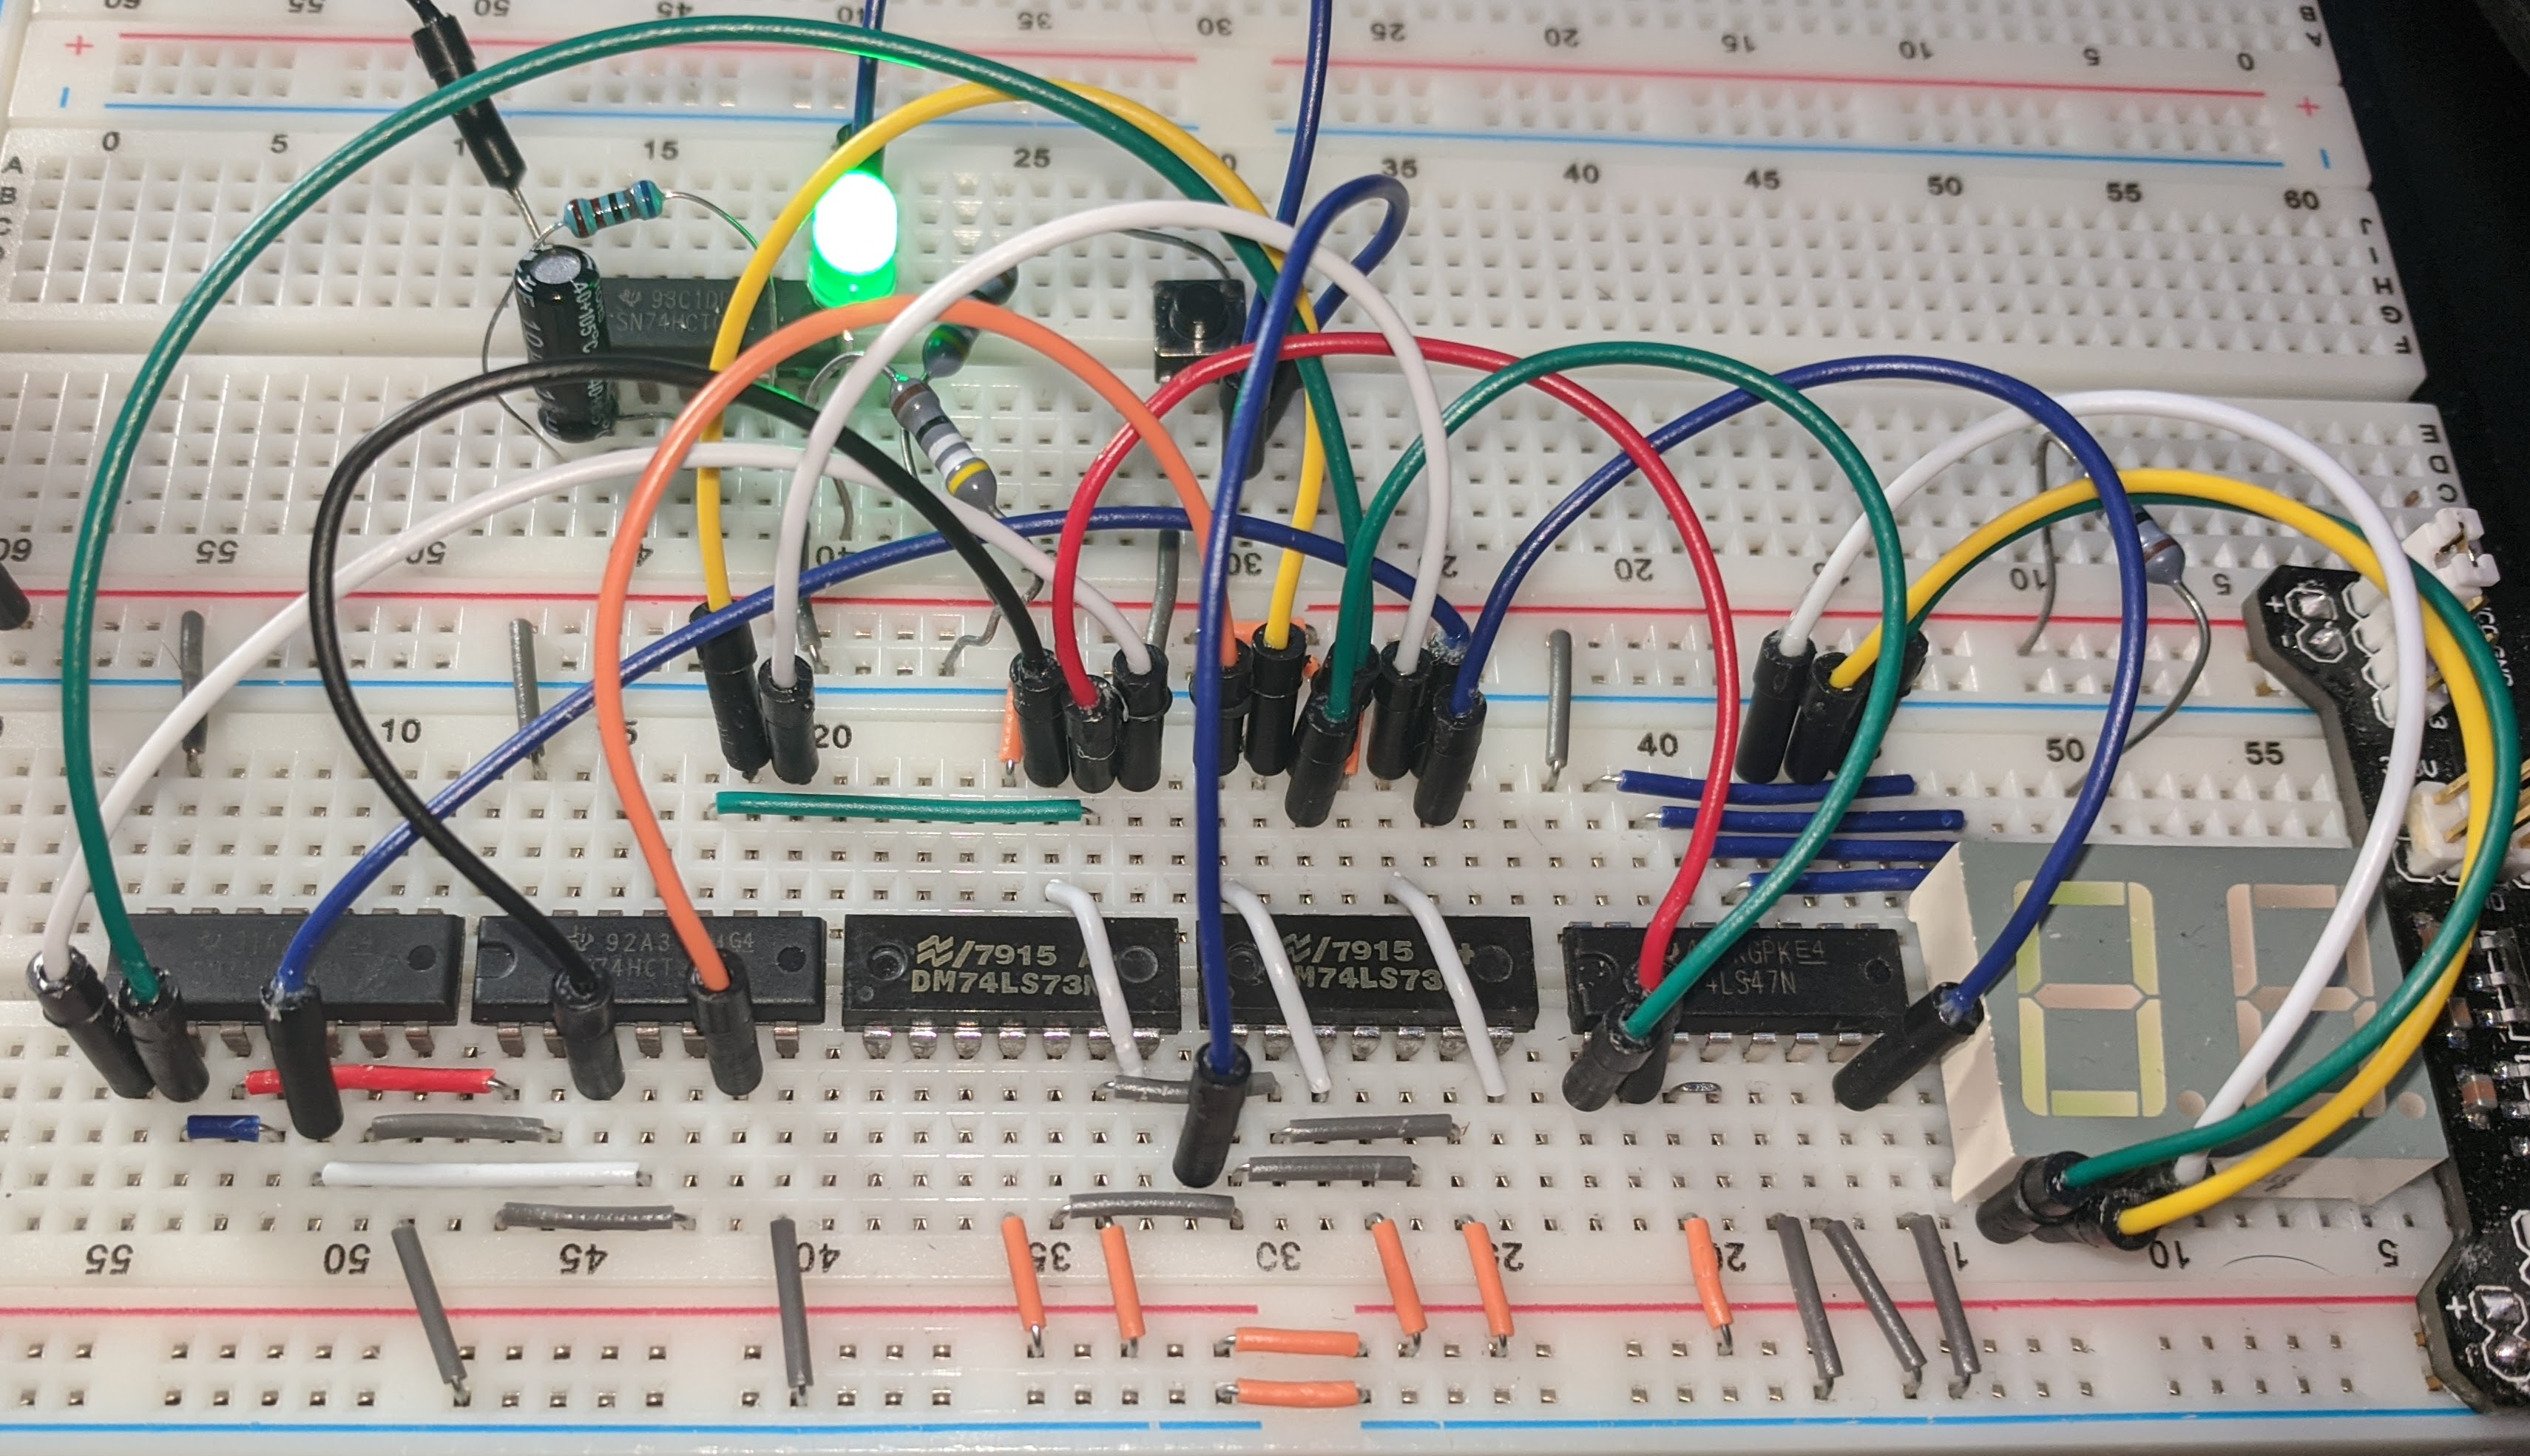
\includegraphics[width=\textwidth]{ECE2300L_Lab12_Counter.jpg}
\end{figure}
\begin{figure}[ht!]
  \centering
  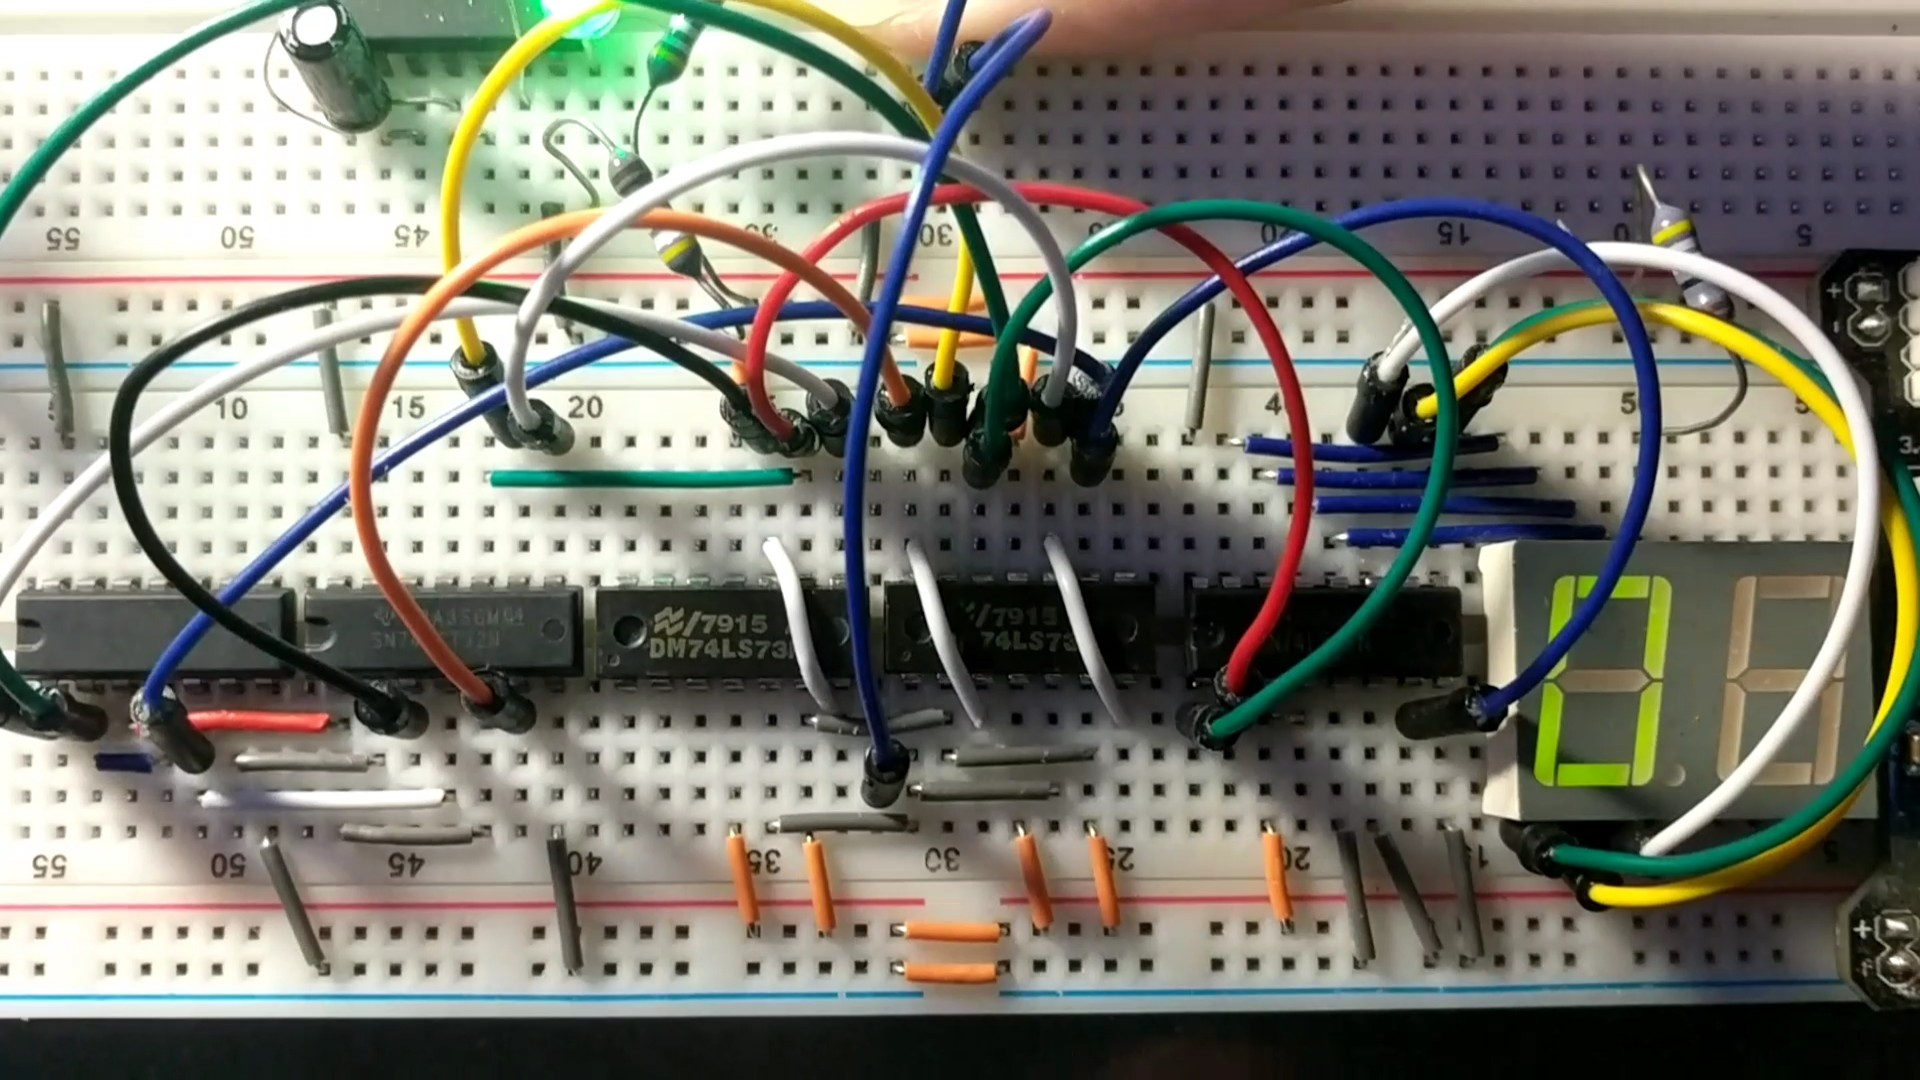
\includegraphics[width=\textwidth]{ECE2300L_Lab12_0.jpg}
\end{figure}
\begin{figure}[ht!]
  \centering
  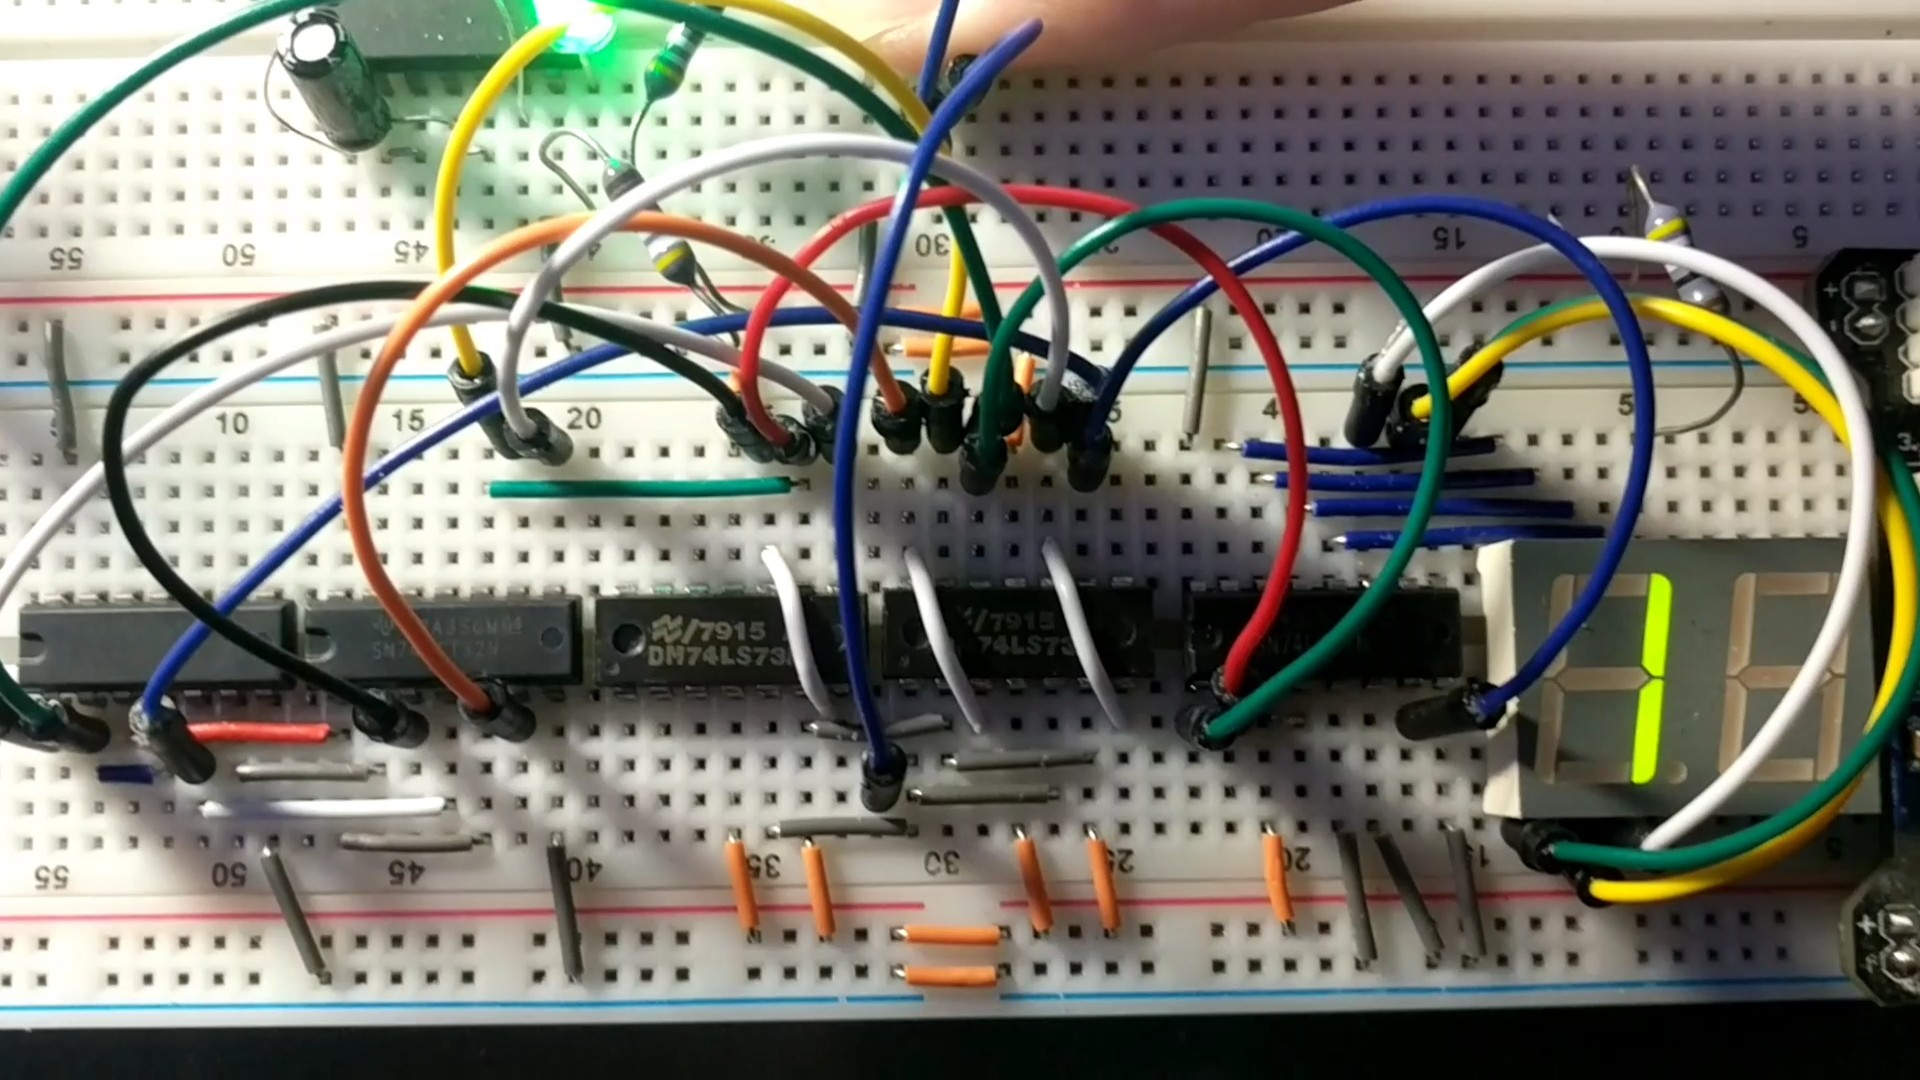
\includegraphics[width=\textwidth]{ECE2300L_Lab12_1.jpg}
\end{figure}
\begin{figure}[ht!]
  \centering
  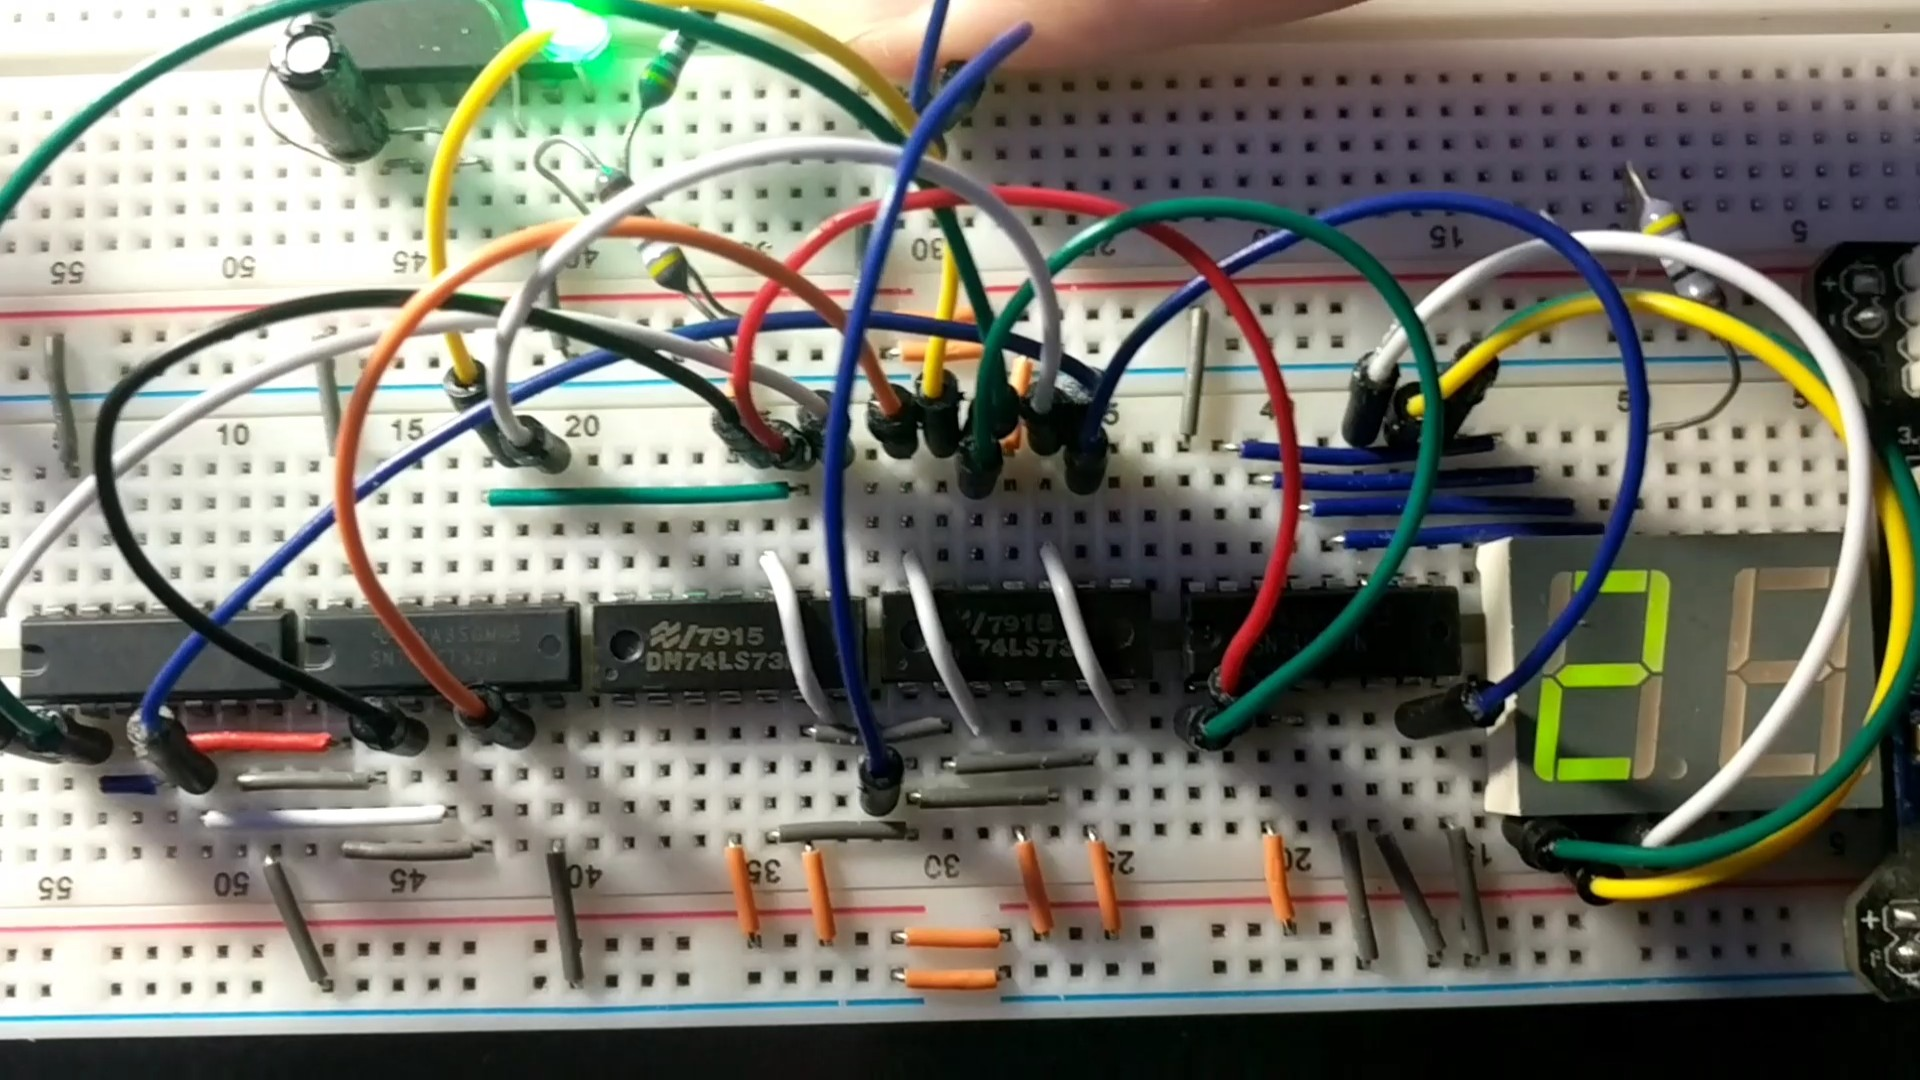
\includegraphics[width=\textwidth]{ECE2300L_Lab12_2.jpg}
\end{figure}
\begin{figure}[ht!]
  \centering
  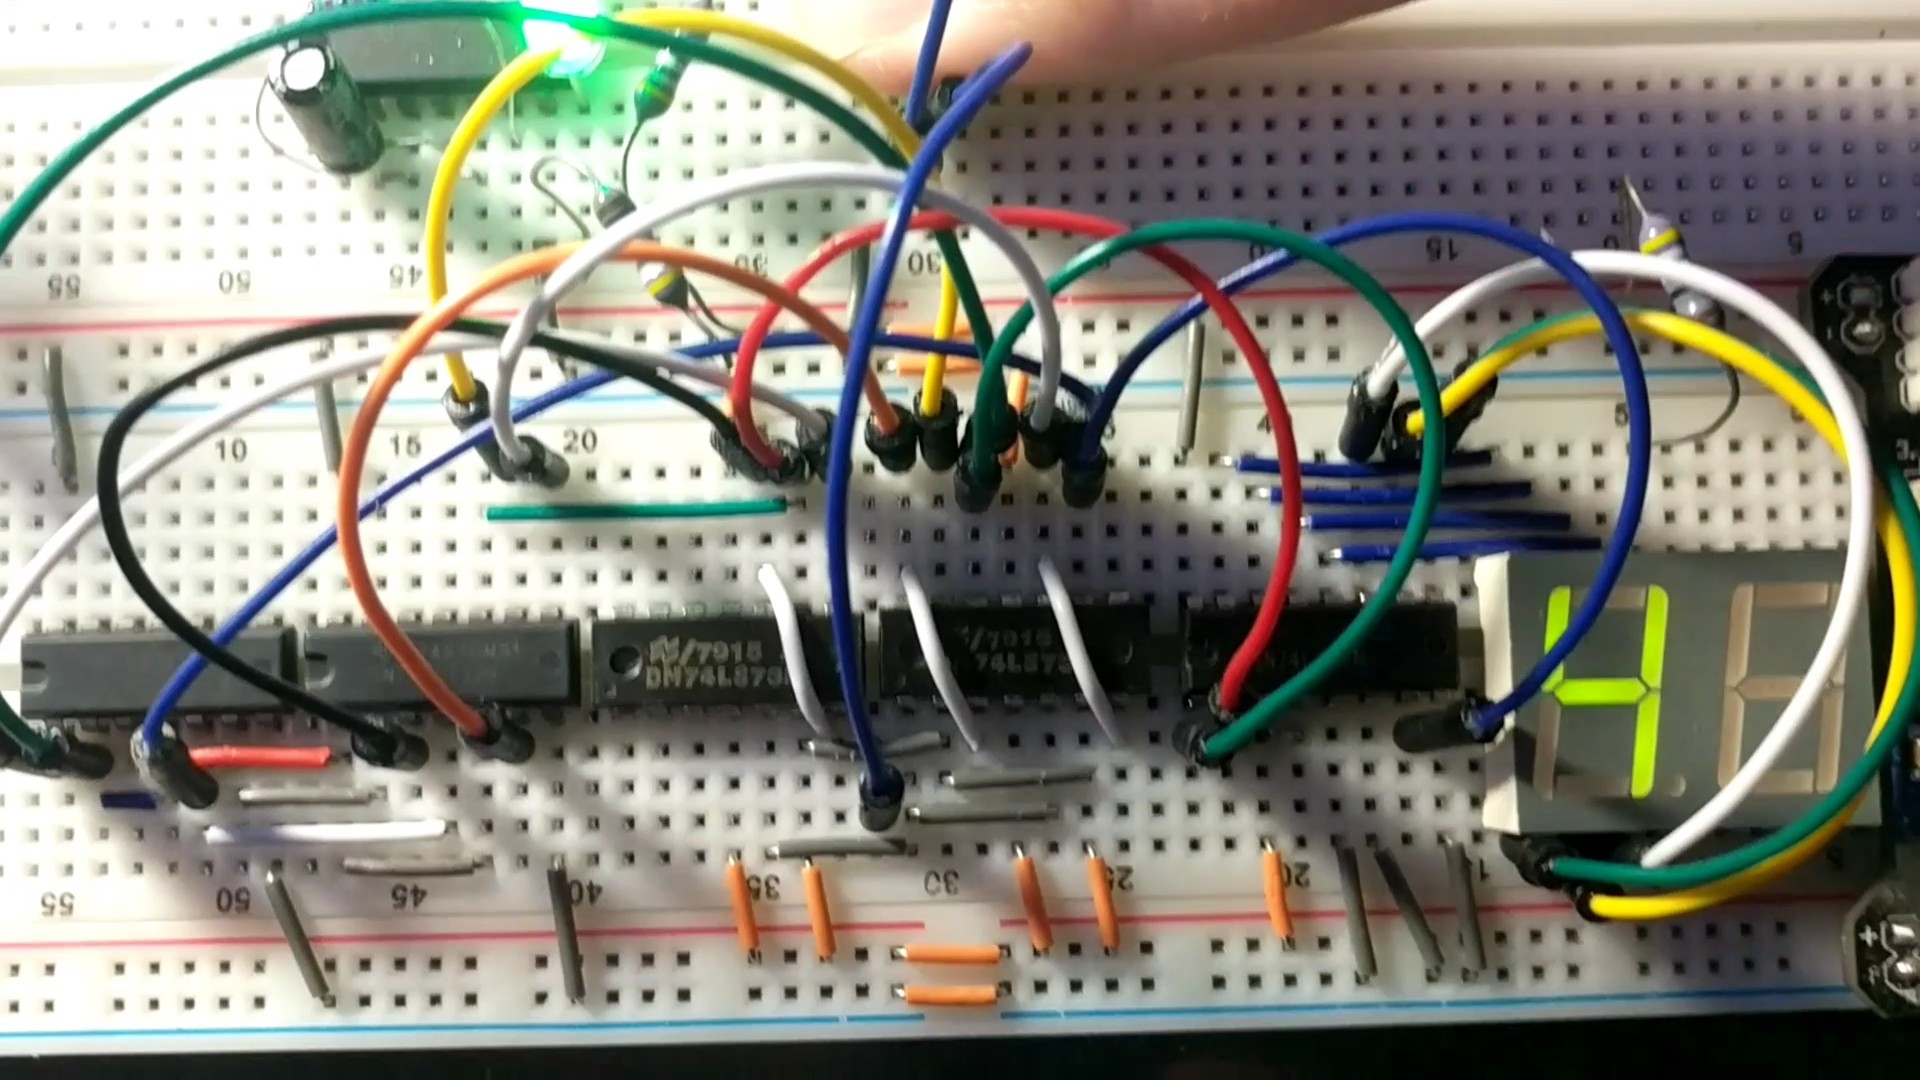
\includegraphics[width=\textwidth]{ECE2300L_Lab12_4.jpg}
\end{figure}
\begin{figure}[ht!]
  \centering
  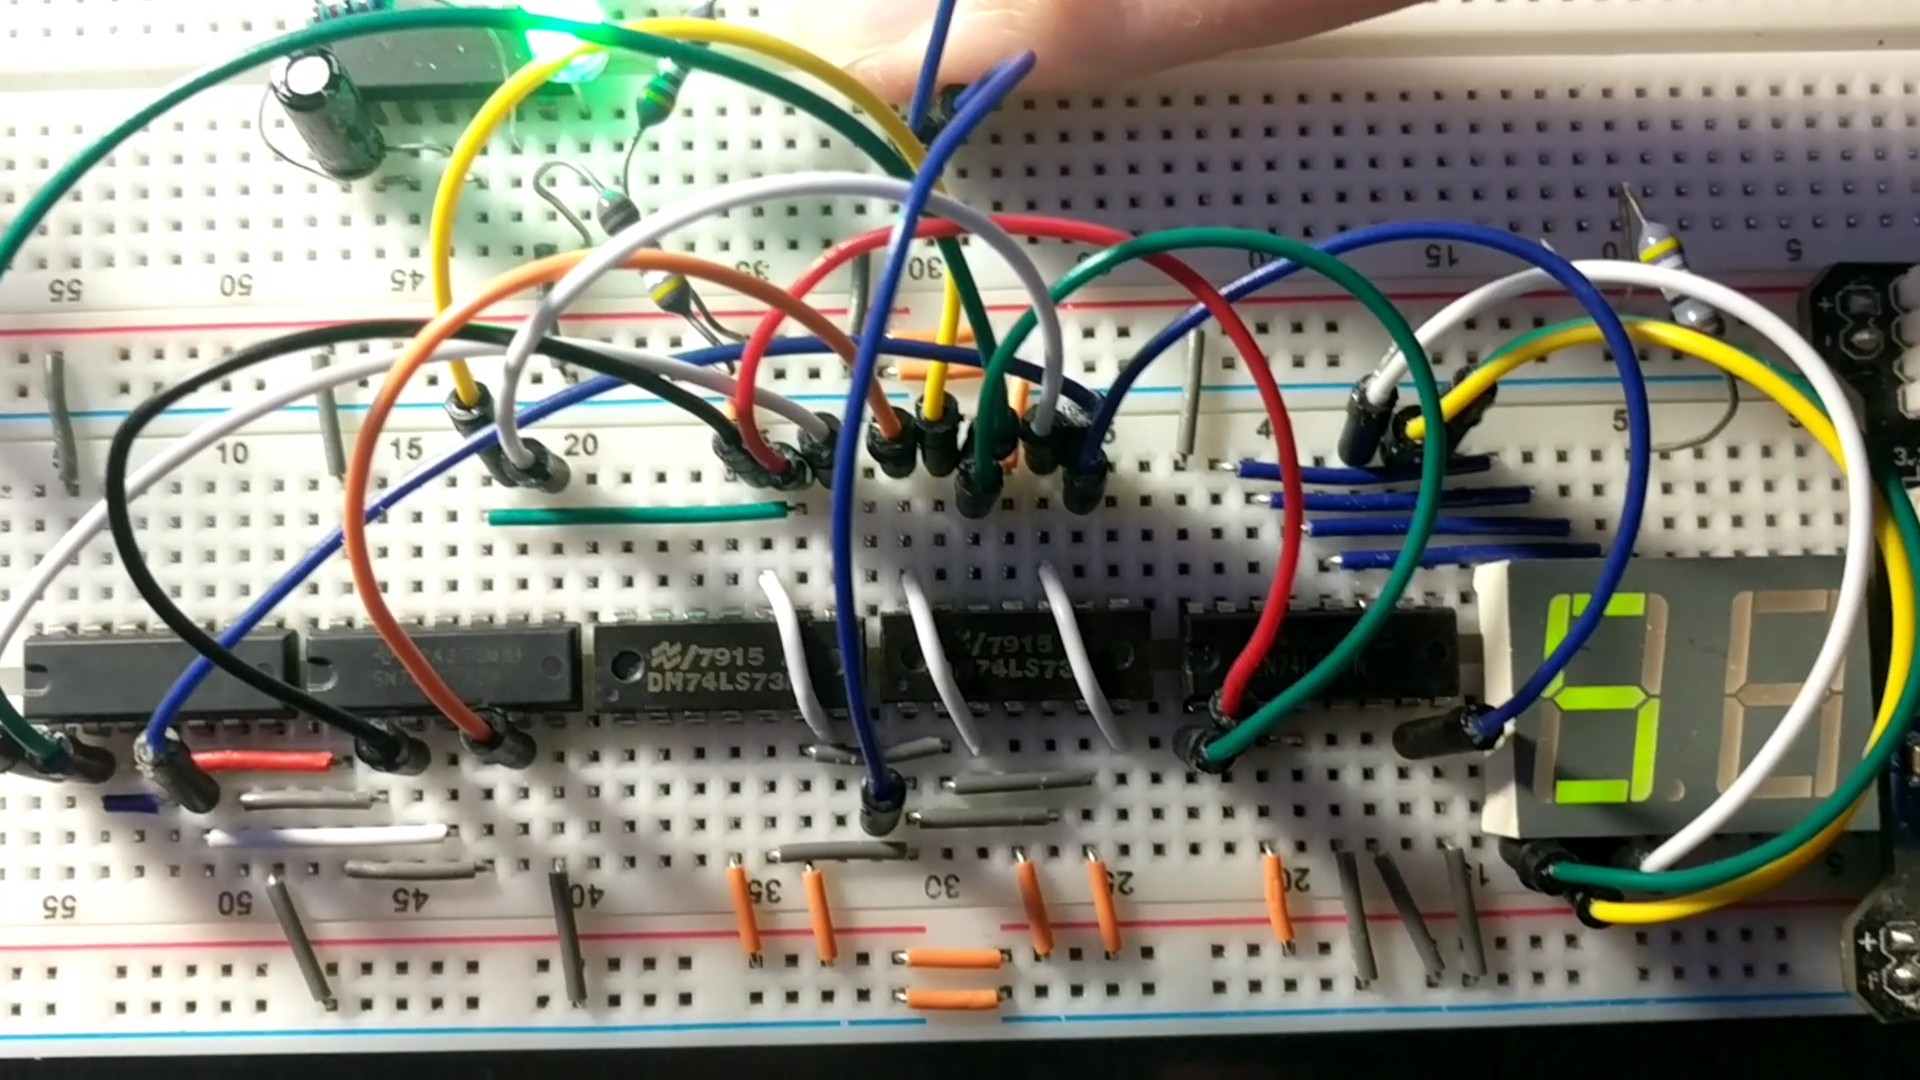
\includegraphics[width=\textwidth]{ECE2300L_Lab12_5.jpg}
\end{figure}
\begin{figure}[ht!]
  \centering
  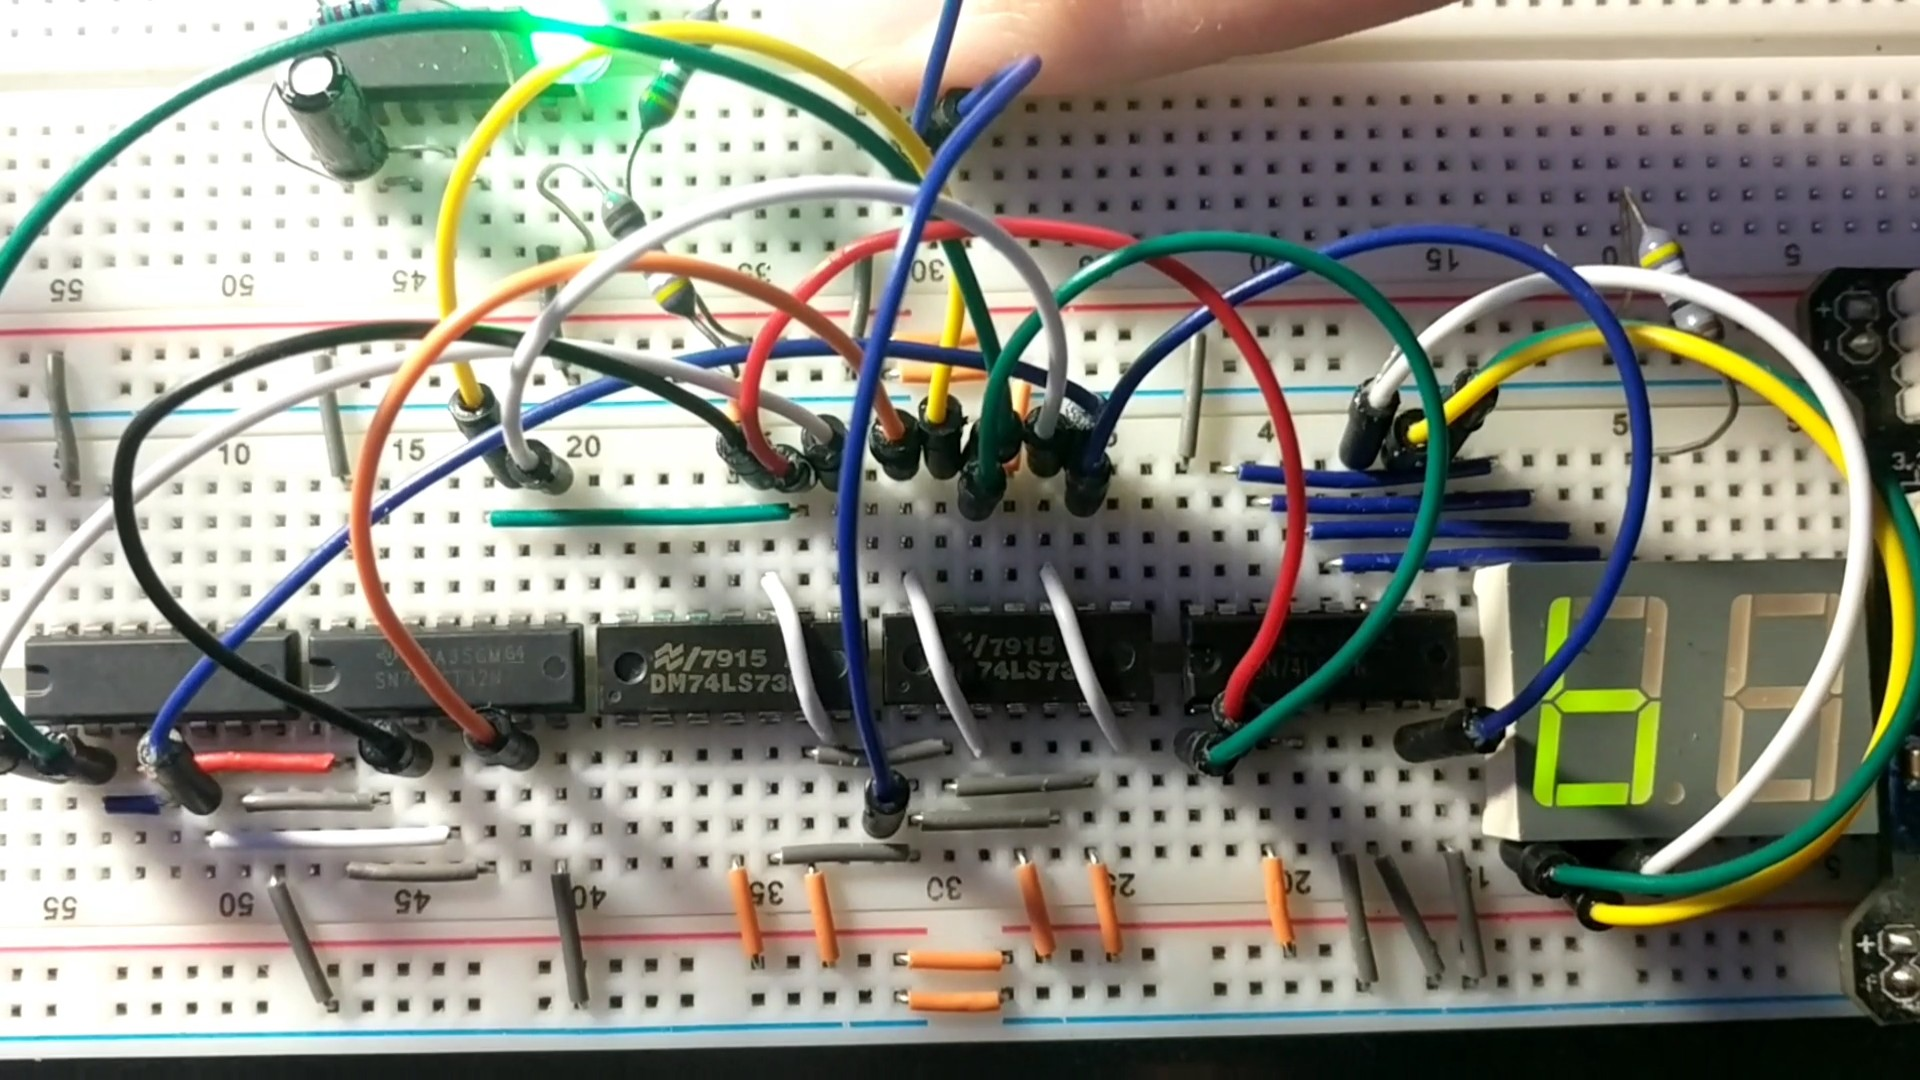
\includegraphics[width=\textwidth]{ECE2300L_Lab12_6.jpg}
\end{figure}
\begin{figure}[ht!]
  \centering
  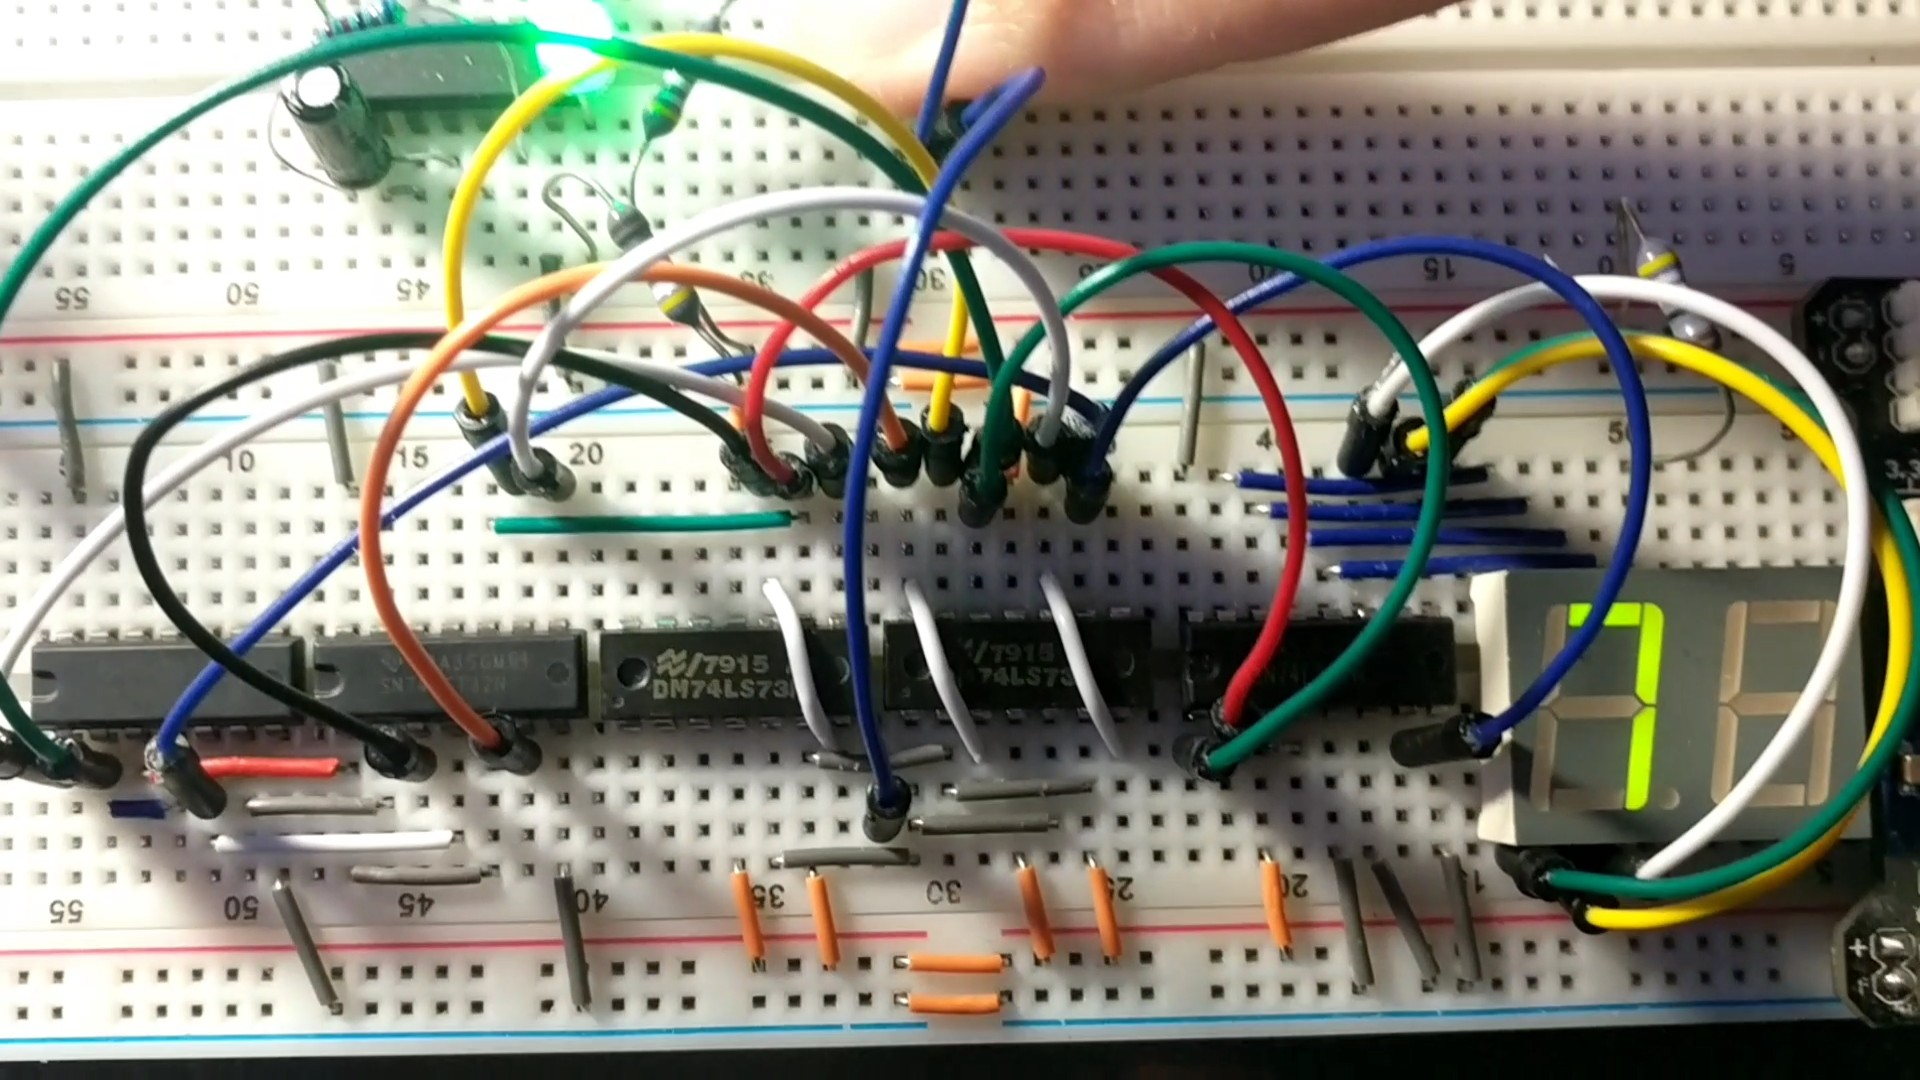
\includegraphics[width=\textwidth]{ECE2300L_Lab12_7.jpg}
\end{figure}
\end{document}
